\documentclass[PMI,VKR]{HSEUniversity}
% Возможные опции: KR или VKR; PI или BI

\title{Dynamic Topic Modeling for Voice Dialogues}
\author{Miakov Timofey Ilich}
\Abstract{}

\bibliography{library.bib}

\begin{document}
\maketitle

\chapter*{Introduction}

Natural Language Processing (NLP) has emerged as a crucial field in computer science, enabling machines to comprehend and respond to human language in a meaningful way. 
Among the various tasks within NLP, dialogue understanding, which involves analyzing and interpreting natural language conversations, has gained significant attention. 
One of the key challenges in dialogue understanding is identifying and tracking different topics discussed throughout the conversation.

Topic modeling is a statistical technique that helps uncover topic structures within textual data. 
Traditional topic modeling approaches, however, suffer from limitations such as topic drift, where the topics change over time, and the inability to capture dynamic relationships between topics. 
In order to analyse time-dependent text corpora, the Dynamic Topic Modeling (DTM) approach is utilised, which will be subjected to further investigation in the forthcoming work.

In this paper, we explore current approaches to (DTM) and apply them to text and audio dialogue datasets. 
Furthermore, we will endeavour to combine several of the most effective open-source methodologies into pipeline from text clustering to topic evolution over time. 
A significant aspect of our research will be to investigate the potential for integrating Large Language Models into our DTM pipeline, with a view to comparing it with other existing solutions.

The quality and performance of the pipeline will be evaluated using specific metrics at both the overall and stage-specific levels. Following this, a comparison will be made with other existing solutions and models.


\section{Relevance of the topic}

Dynamic Topic Modeling is a powerful tool for voice dialogue understanding, offering a dynamic and comprehensive representation of the conversation structure. 
It has the potential to significantly enhance the performance of voice dialogue systems and improve the overall user experience.
In addition, exploring the possibilities of using large language models, which are now showing significant results in many NLP tasks, can further improve the model.


\section{Research Objectives}

The main objectives of the research work is to create and apply Dynamic Topic Modeling pipeline based on LLM for topic extraction for audio and text dialogues. 
To solve this problem, you will need to complete the following tasks 
\begin{enumerate}
    \item The identification of suitable datasets for experiments;
    \item The investigation of the best suitable open-source solutions for speaker diarisation, dialogue clustering, topic extraction and topic evolution;
    \item The exploration of the possibilities of using Large Language Models for some stages and the selection of models suitable for training in limited resources;
    \item The selection of appropriate metrics and measurement of the quality of the approaches used at each stage;
\end{enumerate}

    
\chapter{Literature review}

\section{Transformer architecture}

The main architecture for working with text was Recurrent Neural Networks. However, this approach has several well-known disadvantages:

First of all, RN processes tokens and updates the hidden state sequentially, with this approach, the model begins to forget what happened before or it has to have a huge hidden state.
Secondly, it is very difficult to start distributed training of recurrent networks, because the hidden state at each step must be considered separately.

In order to avoid the issues previously outlined, the article "Attention is all you need" \cite{attention:2017} presented the Transformer architecture and its principal component, 
the Attention Mechanism. The objective of this methodology is to permit the elements of the sequence to be accessed at any time, thereby reducing the loss of information.

\subsection{Self-attention mechanism}

Self-attention represents a key component of the model in which tokens' information interact with each other.
At each stage of the encoder, tokens exchange information with one another, gather contextual data, and refine their previous representations (Figure 2.3). 

For each input token trainable projections $W_Q$, $W_K$, $W_V$ obtained three representations interpreted by humans as a query ($q_i$), a key ($k_i$), and a value ($v_i$).
\begin{itemize}
    \item $q_i$ - query for other tokens about the information;
    \item $k_i$ - keys that will be used to extract information about the token;
    \item $v_i$ - values of information;
\end{itemize}

Next are the attention weights that will be applied to the values from which the important information will be extracted:
\begin{center}
    $Attn_Weights_{i} = softmax(\frac{q_i \cdot k_{1}^T}{C}, \frac{q_i \cdot k_{2}^T}{C}, \dots)$,
\end{center}

where $C$ is some normalization constant.

The Self-Attention result is a weighted sum of Values with coefficients in the form of attention weights. In vectorized form, you can write:

\begin{center}
    $Attention(q, k, v) = softmax(\frac{Q \cdot K^T}{\sqrt{d_k}}) \cdot V $
\end{center}
where $\sqrt[]{d}$ constant of the dimension of $K$ and $V$. 

The figure below shows the complete algorithm for the interaction of Q, K, V.

\begin{figure}[h]
    \centering
    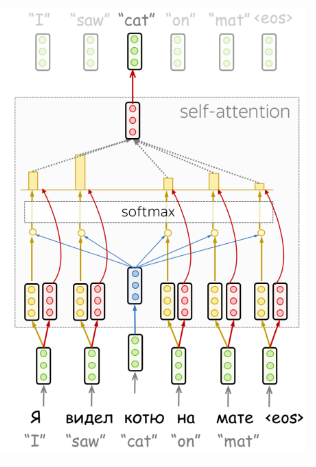
\includegraphics[scale=1]{img/query-key-value.png}
    \caption{Query, Key, Value in Self-Attention mechanism}
\end{figure}

The decoder uses a modified Self-attention mechanism called Masked Self-attention. Because a new sequence is generated in the decoder, the tokens that come after the current one are masked so that the model does not see future tokens and does not rely on information about them. 
Masking leads to the fact that after softmax in the attention mechanism, the probability of future tokens is zero.

\subsection{Multi-head attention}

To cover more information and dependencies, the authors propose Multi-head attention, that use of multiple levels of attention in parallel and the summarisation of the values obtained. 
The figure below illustrates what a multi-head approach looks like:

\begin{figure}[h]
    \centering
    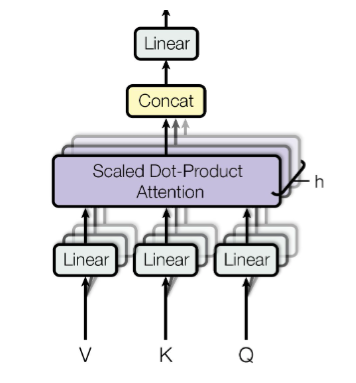
\includegraphics[scale=0.7]{img/multi-head.png}
    \caption{Multi-head Attention mechanism}
\end{figure}

\subsection{Feed Forward Network}

Transformer block also contains feed-forward network consisting of a linear layer and a activation function.
The FFN layer can be expressed as follows:
\begin{center}
    $FFN(x) = act(x \dot W_{1} + b_{1}) \dot W_{2} + b_{2}$, \\    
\end{center}
where $act$ is the activation function such as ReLU = $\max(0, x)$ or more contemporary GELU = $x\Phi(x)$.

\subsection{LayerNorm}

In terms of LayerNorm (Figure 2.3), it is normalizes the vector representation of each sequence in the batch. 
In addition, LayerNorm has trainable parameters, $scale$ and $bias$, which are used after normalization to scale the output of the layer.

\begin{figure}[h]
    \centering
    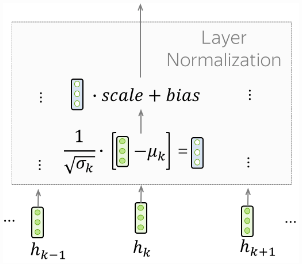
\includegraphics[scale=1]{img/layer_norm.png}
    \caption{LayerNorm слой}
\end{figure}

The application of layer normalisation ensures that all parameters within a given layer exhibit a uniform distribution across all features for a specific input.
The LayerNorm can be expressed as:
\begin{center}
    $y = \frac{x - \mu}{\sqrt{\sigma^{2} + \epsilon}} \odot \gamma + \beta$,
\end{center}
where $\mu$ - mean of last D dimension, $\sigma^2$ - variance of last D dimension, $\gamma$ and $\beta$ - learnable params;
      

\subsection{Positional encodings and Rotary embedding}

Model itself does not understand in which order the input tokens tokens are located. 
Therefore, positional embeddings are added to the tokens, which are designed to show the model the input order of the elements.
Positional embeddings are given by formulas:
\begin{center}
    $PE_{position, 2i} = \sin(\frac{position}{10000^{2i/d_{model}}})$, \\
    $PE_{position, 2i+1} = \cos(\frac{position}{10000^{2i/d_{model}}})$, \\
\end{center}

Each measure of position encoding corresponds to a sin wave, and the wavelengths form a geometric progression from $2\pi$ to 10,000$\cdot 2\pi$.

\begin{figure}[h]
    \centering
    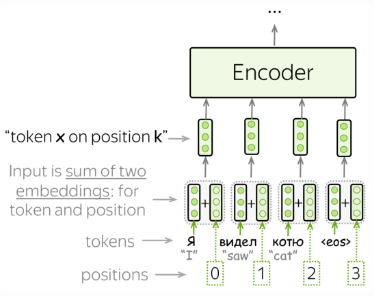
\includegraphics[scale=1]{img/pos_encoding.png}
    \caption{Positional encoding}
\end{figure}

A newer version of positional encoding is Rotary Positional Embeddings \cite{rotary:2021}.
Rotary position embedding represents a distinct approach to incorporating relative position information into the attention matrix. 
This approach differs from other approaches in that it first multiplies queries and keys with a rotation matrix. This rotation matrix is a function of absolute position. 
Calculating the inner products of rotated queries $W_Q$ and keys $W_K$ results in an attention matrix that is a function of relative position information only.

In order to illustrate the concept, we will consider an examples with two features at position $m$.
\begin{center}
    $RoPE(x_1, x_2) =   \begin{pmatrix}
                            \cos m\theta & -\sin m\theta\\
                            \sin\theta & \cos m\theta
                        \end{pmatrix} 
                        \begin{pmatrix}
                            x_1 \\
                            x_2
                        \end{pmatrix} 
                        \begin{pmatrix}
                            x_1 \cos m\theta - x_2\sin m\theta\\
                            x_2 \cos m\theta + x_1\sin m\theta
                        \end{pmatrix},
    $
\end{center}
where $\theta$ is a constant angle.


\section{Transformer based models}

Several models based on the Transformer architecture will be required in the work at different stages. 
More specifically, text clustering will require an encoder for text information based on BERT, and LLM will be used for topic processing.

\subsection{BERT}

The BERT is a language model based on the transformer architecture, that was first introduced in the article BERT: Pre-training of Deep Bidirectional Transformers for Language Understanding\cite{bert:2018}.  
From an architectural point of view, BERT consists of 12 encoder blocks, including a Self-Attention mechanism, Normalization and Feed-forward layers.

\begin{figure}[h]
    \centering
    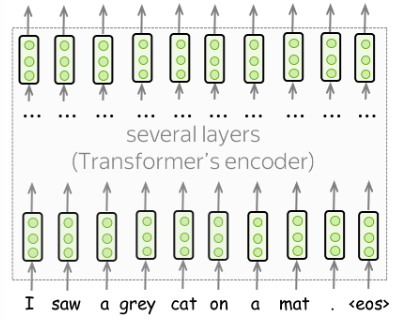
\includegraphics[scale=0.8]{img/bert.png}
    \caption{BERT architecture}
\end{figure}

\textbf{BERT has two pretrain objective} described in article: \\
The first objective of the training process is the masked language modelling (MLM). 
During the training phase of MLM, the following occurs:

\begin{itemize}
    \item A number of tokens are selected with a probability of 15\% for each token.
    \item The selected tokens are replaced by [MASK] with a probability of 80\%, a random token with a probability of 15\% and remain unchanged with a probability of 10\%.
    \item The model must predict the original token.
\end{itemize}

Secondly, Next Sentence Prediction (NSP) pretraining task is a binary classification task. 
In order to understand relationship between two sentences, BERT training process also uses next sentence prediction.
During training the model gets as input pairs of sentences and it learns to predict if the second sentence is the next sentence in the original text as well. 
The training dataset presented in the original paper states that when trained, 50\% of the examples contain related sentences extracted from the training texts, while the remaining 50\% contain a random pair of sentences.\\


\textbf{LLM} is a type of artificial intelligence(AI) algorithm that use deep learning techniques and massively large data sets to understand, summarize, generate, and predict new content. 
LLMs are trained with immense amounts of data and use self-supervised learning to predict the next token in a sentence, given the surrounding context. 
Once an LLM has been trained, it can be fine-tuned for a wide range of NLP tasks, including generating and classifying text, answering questions.
The following section will examine the main LLMs used in the experiments: LLaMA, Mistral, Qwen.

\subsection{LLaMA}

In July 2023, an open-source collection of models, called LLaMA2 \cite{llama:2023}, was released by Mata AI Team. The collection consists of models with 7B and 70B parameters.

In order to create a collection of LLaMA 2 models, the authors employed the architecture of an optimised auto-regressive transformer (Touvron et al.(2023)) with RMSNorm normalisation, Rotary Embeddings and SwiGLU activation function in FFN, but implemented a number of alterations with the intention of enhancing the quality of the model and its performance, such as:
\begin{itemize}
    \item Meticulous data preparation
    \item Larger dataset
    \item Increased the length of the context in compare with earlier approaches
    \item Incorporation of grouped-query attention (GQA)
\end{itemize}   

\textbf{Grouped-query attention} can be thought of as a way to optimize the attention mechanism in transformer-based models. 
Instead of computing attention for each query independently, GQA groups queries together and computes their attention jointly. This reduces the number of attention computations, leading to faster inference times.

The GQA method has been applied to speed up inference on large language models without significantly sacrificing quality. 
It's a promising technique for improving the efficiency of transformer models, particularly in the context of generative AI.

\begin{figure}[h]
    \centering
    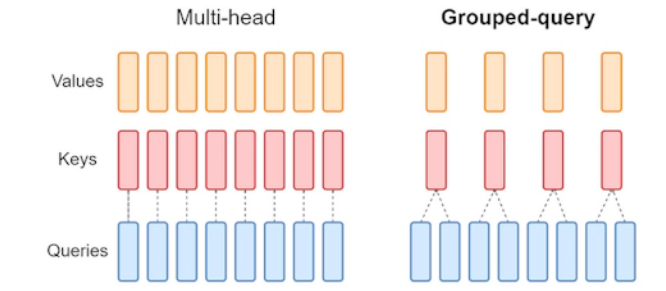
\includegraphics[scale=1]{img/gqa.png}
    \caption{Self-attention and Grouped-query attention}
\end{figure} 

\newpage
In april 2024 was released LLaMA3 8B and 70B models with some new features: larger tokenizer vocabulary 128k agains 32k, the dataset for pre-training contains 8 times more sampels on over 15 trillion tokens on a new mix of publicly available online data.   


\subsection{Mistral}

In September 2023, the MistralAI \cite{mistral:2023} team introduced the Mistral 7B model, which has been designed for high performance and efficiency. 
In comparison to the 13B Llama 2, the Mistral 7B model has demonstrated superior performance in all benchmarks related to reasoning, mathematics, and code generation. 
The Mistral 7B model employs grouped-query attention (GQA) for rapid inference and sliding window attention (SWA) for handling long sequences at a reduced cost.

As other models, Mistral is a transformer based model. However, it differs from the Llama model in several key respects.
\begin{itemize}
    \item Sliding Window Attention (SWA): This method allows the model to attend to information beyond a set window size by leveraging the stacked layers of a transformer. 
    With a window size of 4096, it can attend to around 131K tokens. 
    \item Rolling Buffer Cache: It is limits the size of the cache using a rolling buffer. The cache has a fixed size, and as new data is added, older data is overwritten once the cache exceeds its size. 
    This method reduces the memory usage of the cache by 8x for sequences of 32k tokens without compromising the quality of the model.
    \item In the context of sequence generation, the model employs a process of pre-filling and chunking. 
    This involves the prediction of tokens in a sequential manner, given that each token is contingent upon the previous one. However, given that the prompts are known in advance, the cache can be pre-filled with them. 
    In the event that a prompt is of a considerable length, it can be divided into smaller units, with the cache being filled in this manner. 
    The attention mask operates over both the cache and the chunk
\end{itemize}

\subsection{Qwen}

The Qwen LLMs have been extensively trained on up to 3 trillion tokens of diverse text and code examples from a wide range of domains. 
Qwen demonstrate superior performance in various downstream tasks.

In terms of architecture: model based on LLaMA, activation function is SwiGLU, Rotary Embeddings, Pre-Norm and RMSNorm instead LayerNorm. 

The pre-training phase involves learning vast amounts of data to gain a comprehensive understanding of the world and its various complexities. 
This includes not only basic language skills, but also advanced skills such as arithmetic, coding and reasoning. 
In this section we introduce the data, model design and scaling, and the extensive evaluation results on benchmark datasets.

The Qwen Series encompasses models that employ SFT and RLHF to align Qwen with human preference. 
Consequently, the Qwen-Chat and its enhanced variant, the Qwen-Chat-RLHF, have been developed. Furthermore, we have created bespoke models for coding and mathematics.

\begin{figure}[h]
    \centering
    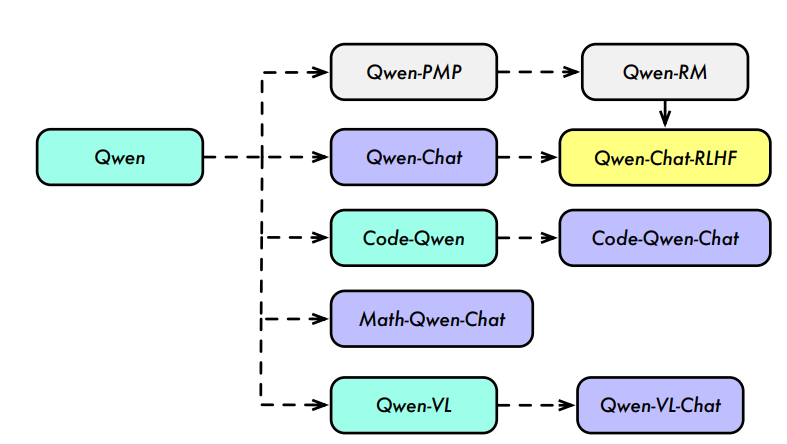
\includegraphics[scale=1]{img/qwen.png}
    \caption{Qwen Series}
\end{figure} 

For now, there are 5 models of different sizes, 4 of which are opensourced. Specially, Qwen-1.8B, Qwen-7B, Qwen-14B, and Qwen-72B.

\section{Speaker diarization}

Since one of the significant tasks is to use DTM for audio dialogues, the first, but optional, stage of our pipeline will be a model for speaker diarization. 

Speaker diarisation is the process of automatically segmenting and identifying different speakers in an audio recording. 
The goal of speaker diarisation is to divide the audio stream into non-homogeneous segments, each segment corresponding to a specific speaker or speaker turn.

The fundamental process of building a speaker diarization system involves the following steps:

\begin{itemize}
    \item Segmentation: The audio recording is divided into differente segments based on conditions like silence, pauses, and changes in speaker turns.
    \item Speaker Embedding: Embeddings are extracted for each segment to represent the speech features of unique speaker.
    \item Clustering: The extracted embeddings are clustered based on similarity, with segments from the same speaker forming a single cluster.
    \item Labeling: Once the clustering is complete, each segment is assigned a label representing the speaker's identity. Segments in the same cluster are assigned the same label, indicating they belong to the same speaker.
\end{itemize}

As ASR model for this stage, we will look at the Whisper \cite{whisper:2022} model from OpenAI.

\subsection{Whisper}

Whisper is an automatic speech recognition (ASR) system trained on 680,000 hours of multilingual and multitask supervised data collected from the web. 
We show that the use of such a large and diverse dataset leads to improved robustness to accents, background noise and technical language. Moreover, it enables transcription in multiple languages, as well as translation from those languages into English. 
We are open-sourcing models and inference code to serve as a foundation for building useful applications and for further research on robust speech processing.

\begin{figure}[h]
    \centering
    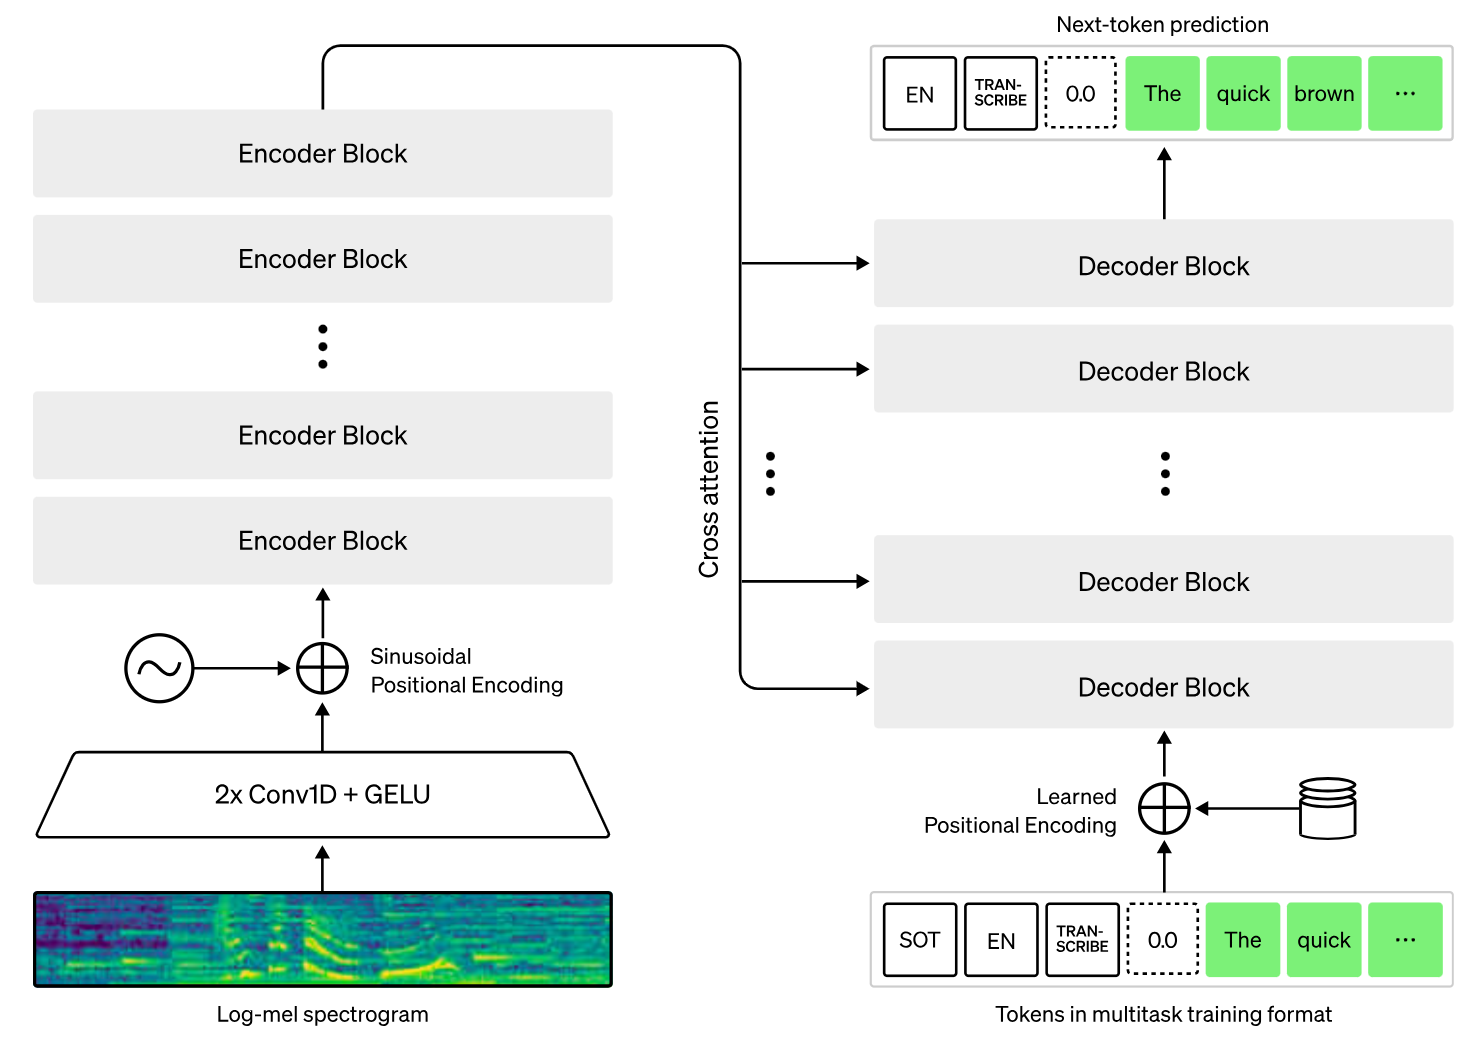
\includegraphics[scale=0.7]{img/whisper.png}
    \caption{Whisper architecture}
\end{figure}

The Whisper architecture is a simple end-to-end approach, implemented as an encoder-decoder Transformer. 
Input audio is split into 30-second chunks, converted into a log-Mel spectrogram, and then passed into an encoder. 
A decoder is trained to predict the corresponding text caption, intermixed with special tokens that direct the single model to perform tasks such as language identification, phrase-level timestamps, multilingual speech transcription, and to-English speech translation.

\section{Improving Utterance-Pair Coherence Scoring}
\label{seg}

The dialogue segmentation stage represents the initial stage for textual type of data. 
The result is a set of utterance indices that indicate the beginning of a thematically related group. 

In accordance with the majority of previous studies, we have utilise the best open-source solution based on the presented in papers metrics. 
It is algorithm from Improving Unsupervised Dialogue Topic Segmentation with Utterance-Pair Coherence Scoring \cite{depthscore:2021} 
Let us now examine the algorithm in greater detail. 

\subsection{BERT for coherence scoring}

In terms of our approach to topic segmentation, authors utilise Next Sentence Prediction (NSP) BERT as the encoder, due to the similar type of task. 
Input of both tasks an utterances, with the objective of predicting the appropriate next sentence, which should be topically related. 

In more detail, the positive instances $(s_{i}, s_{t+i})$ and negative instances $(s_{i}, s_{t-i})$ use in the model's fine-tuning stage in the form described below: 
\begin{center}
    $[CLS] s_{i} [SEP] s_{t+/-i} [SEP]$,
\end{center}
where the symbols $[CLS]$ and $[SEP]$ represent special tokens in BERT. 

In order to indicate the thematic similarity of two statements in a dialogue, the $[CLS]$ token is employed, which performs a similar role in the usual BERT. 
The resulting value is subjected to a linear dictionary and a final similarity value is obtained, which is then utilised to calculate Coherence scores.

\subsection{Depth Scores}

With the help of a fine-tuned BERT (the training algorithm is described above) coherence scores $c_i$, where $i \in [0, n - 1]$ are calculate. According to texttiling algorithm description $c_i$ indicates the topical relatedness of the two adjacent utterances.
The model uses the obtained values as base values, but processes them for final predictions and gets Depth scores $ds_i$, where $i \in [0, n - 1]$  - measuring the sharpness of a valley.

The depth score is calculated as shows below: 
\begin{center}
    $D_{pi} = \frac{h_{l}(i) + h_{r}(i) - 2 \cdot c_{i}}{2}$,
\end{center}
where $h_{l}, h_{r}$ - the highest cs for $i$ pair in choosen range.

The greater the depth score between two statements, the less likely it is that they share a thematic relationship. 
To identify the pairs along which the boundaries of the thematic segments lie, the threshold value is calculated as follows: $threshold = \mu - \frac{\sigma}{2}$, where $\mu$ is the average value and $\sigma$ is the standard deviation. Pairs with a depth score above the $threshold$ value will be choosen as boundaries.


\section{Evaluation Metrics}

\subsection{Speaker diarization}

The standard metric for speaker diarization problem is the Diarization error rate \:
This metric computes the error in diarization in terms of a duration ratio, which means that a perfectly aligned hypothesis and reference diarization would result in DER=0. It sums up 3 error:
\begin{itemize}
    \item False Alarm - speech segment predicted where there is no speaker. It is error from ASR models.
    \item Missed Detection - no speech detected where there is a speaker. It is error from ASR models.
    \item Confusion	Speech - the wrong cluster. It is error from the clustering model
\end{itemize}

\begin{figure}[h]
    \centering
    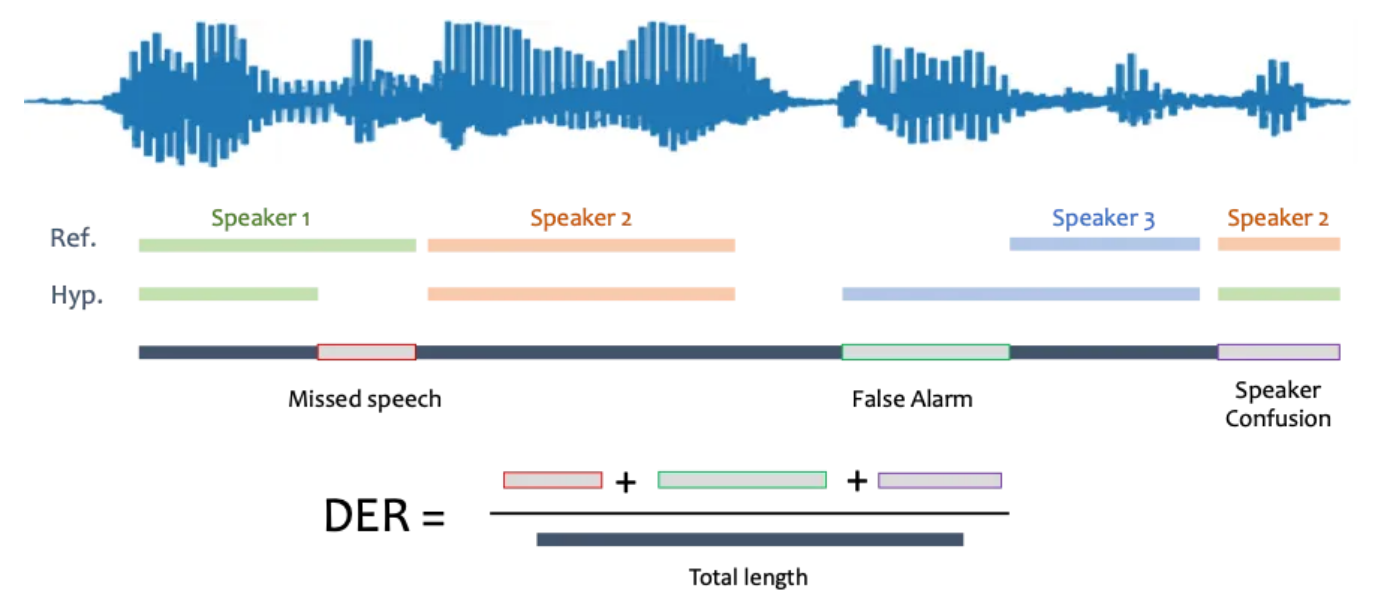
\includegraphics[scale=0.8]{img/der.png}
    \caption{Diarization error rate }
\end{figure}

Mathematically, the metric can be written: 
\begin{center}
    $DER = \frac{False Alarm  +  Missed Detection  +  Confusion}{Total}$    
\end{center}

\subsection{Dialogue segmentation}

After defining the basic segmentation algorithm, it is worth talking about evaluation metrics for this stage:
\begin{itemize}
    \item \textbf{F1}\\
    Given that this is a binary classification problem, it is tempting to use Precision and Recall, and their combination $F_{\beta}$ score as an evaluation metric. \\ 
     - Metric is defined as the boundaries ratio identified as true boundaries; \\
       $Precision = \frac{true \: positive}{true \: positive + false \: positive}$ \\
     - Recall is defined as the true boundaries ratio identified by the model. \\
       $Recall = \frac{true \: positive}{true \: positive + false \: negative}$ \\
    $F_{\beta}$ score is defined as the weighted harmonic mean of precision and recall: \\
    $F_{\beta} = (1 + \beta^{2}) \cdot \frac{precision \cdot recall}{(\beta^{2} \cdot precision) + recall}$
    \item \textbf{Pk score} \cite{pk:1999} is uses the sliding window method and counts the number of discrepancies between the ends of the predicted segments and the true segments. The final score is the counter divided by the number of measurements. The lower the value, the better.
    \item In \textbf{WindowDiff} \cite{wd:2002} this algorithm, for each position of a sliding window of size k, comparing the number of boundaries in the ground truth with the number of boundaries predicted by the Topic Segmentation model. The lower the value, the better.\\
    $WD(pred, true) = \frac{1}{N - k}\sum_{i = 1}^{N - k}(\left\lvert bounds(true_{i}, true_{i + k}) - bounds(pred_{i}, pred_{i + k})\right\rvert > 0)$, \\ 
    where $bounds(s, s + i)$ is the number of boundaries between $i$ and $j$ positions, $N$ - number of sentences in the text.
\end{itemize} 

\subsection{Topic extraction}

As for the quality evaluation of the extracted topics, we will use two metrics: Topic coherence and Topic diversity
\begin{itemize}
    \item \textbf{Topic diversity} \cite{topicdiversity:2019} is a metric that assesses the ratio of unique keywords across all topic representations. This metric is used to measure the capabilities of a topic model covering a wide range of topics. The diversity score is a value between 0 and 1, with a score of 0 indicating repetitive topics and a score of 1 indicating diverse topics.
    \item \textbf{Topic coherence} \cite{topiccoh:2009} is a measure of the degree of interconnection of words within a topic. In our experiments, we employed normalized point-to-point mutual information (PMI) as a metric for thematic consistency. A higher score for a given name indicates greater consistency, with an absolute correlation estimated at 1 point.
\end{itemize}


\chapter{Methodology}

\section{Pipeline configuration}

The pipeline of dynamic thematic modelling of audio dialogues, which will be considered in this paper, is divided into several main stages. 
These include ASR, dialogue segmentation, topic extraction and topic evolution. 

\begin{figure}[h]
    \centering
    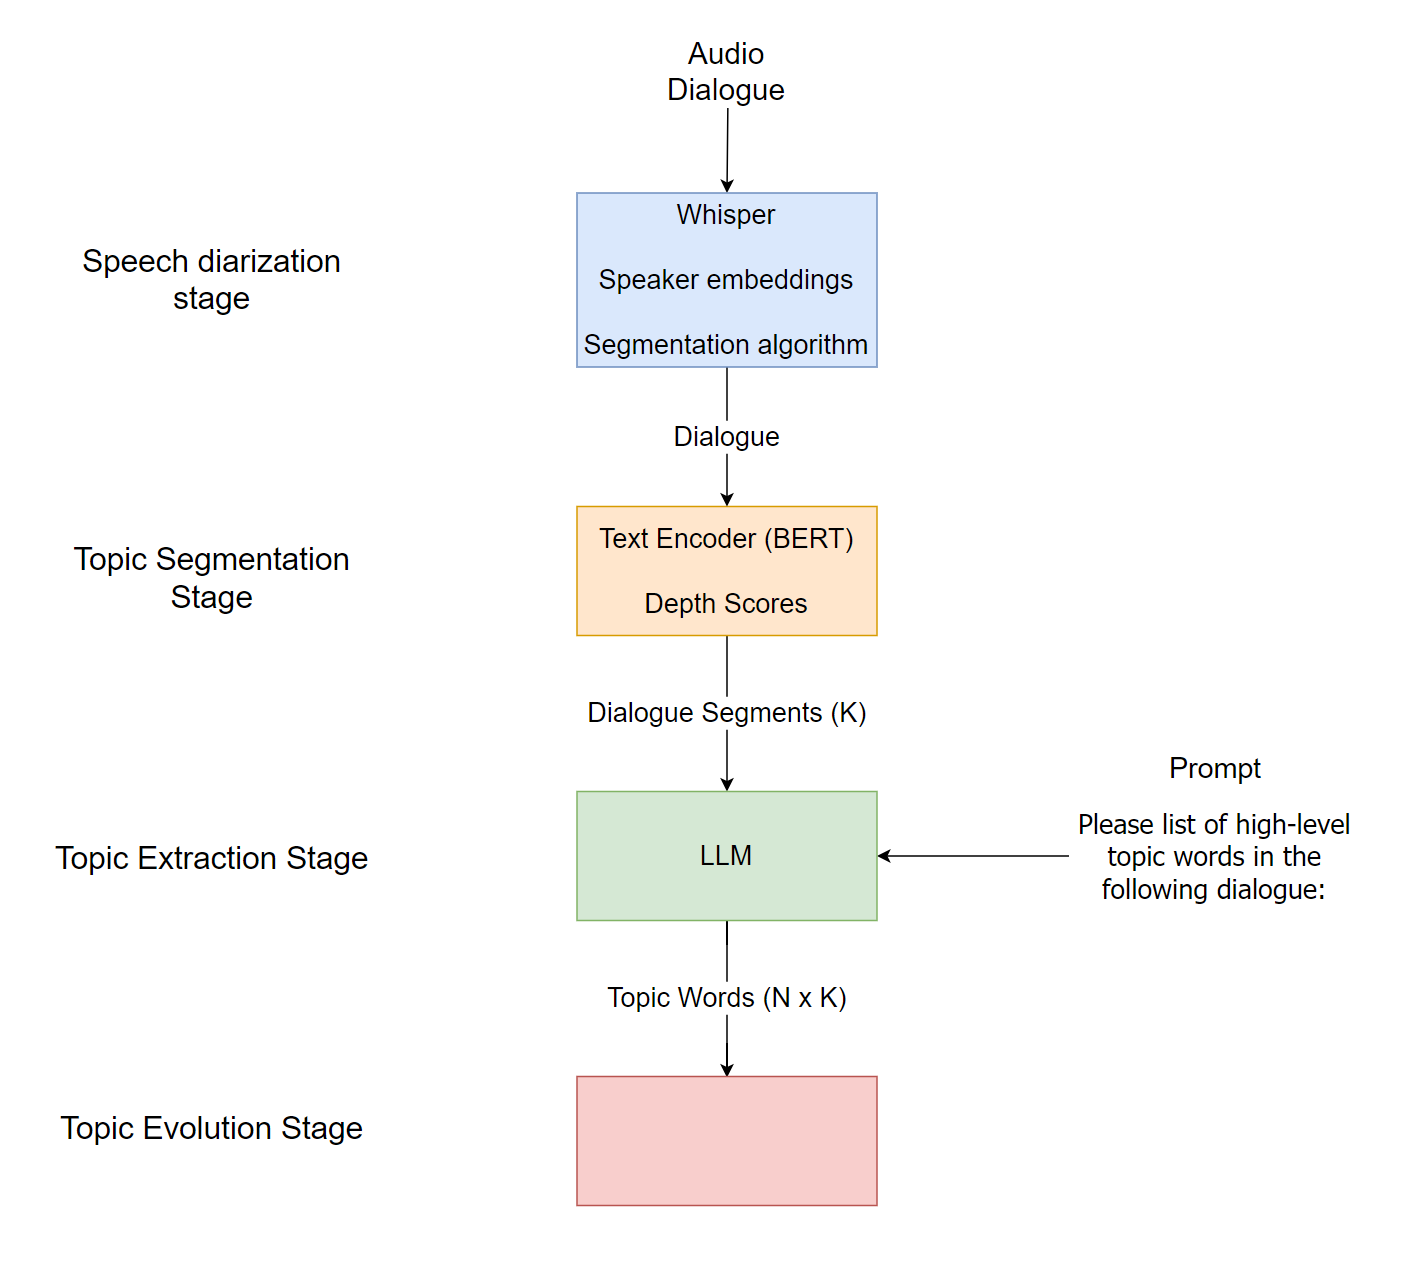
\includegraphics[scale=0.7]{img/pipeline.png}
    \caption{DTM pipeline}
\end{figure}

All the models in the pipeline were taken from the \href{https://huggingface.co/}{HuggingFace} hub. 
Tools from \href{https://huggingface.co/docs/transformers/index}{transformers}, which is also part of HuggingFace, 
will be used to create the pipeline.

\section{Speaker Diarization}

The first optional stage is the Speaker Diarization. 
For audio dialogues, text is extracted from the audio track before topic segmentation. 
For this stage we use:
\begin{itemize}
    \item OpenAI Whisper \\
    Link to model: \href{https://huggingface.co/openai/whisper-large-v3}{whisper-large-v3};
    \item pyannote - speaker diarization library \cite{pyannote:2023} \\
    Link to model: \href{https://github.com/pyannote/pyannote-audio}{[pyannote]};
\end{itemize} 

\section{Dialogue Segmentation}

The algorithm \ref{seg} will be used to dialogues segmentation. 
The implementation of the algorithm will be taken from the \href{https://github.com/lxing532/Dialogue-Topic-Segmenter}{official github repository}. 
Part of the code with the model inference will be adapted to the pipeline.

\section{Topic Extraction}

The next stage in the pipeline is topic extraction. At this stage, $n$ topics will be extracted from each segment in the dialogues. 
At this stage, past approaches have used probabilistic or embedding approaches, like BertTopic \cite{berttopic:2022}. 
In our work, we will apply a generative approach using Large Language models, as in PromptTopic \cite{prompttopic:2023}.

We will try several Large Language Models:
\begin{itemize}
    \item MetaAI LLaMA3 8b \\
    Link to model: \href{https://huggingface.co/meta-llama/Meta-Llama-3-8B-Instruct}{meta-llama3-8b}
    \item Qwen1.5 7b \\
    Link to model: \href{https://huggingface.co/Qwen/Qwen1.5-7B-Chat}{Qwen1.5 7B}
    \item Mistral 7b \\
    Link to model: \href{https://huggingface.co/mistralai/Mistral-7B-Instruct-v0.1}{Mistral 7B}
\end{itemize}  

The prompt for LLM will look like this:

\begin{lstlisting}
    <|user|> 
    <dialogue> 
    Please list of high-level topic words 
    in the following dialogue:
    <|assistant|>
\end{lstlisting}

The appearance of the keywords <|user|>, <|assistant|> dependes on type of LLM.

\section{Topic Evolution}




\chapter{Experiments}

The experiments will be divided into stages, with each stage accompanied by a description of the stage and the algorithms used. 
This description is included in the theoretical part of the work.

\section{Experiments settings}

\textbf{Datasets}
For the experiments we will use two types of datasets: text dialogues and audio dialogues. 
For text dialogues, we will use tiage, compiled from the personal chat corpus and manually annotated, and superdialseg, compiled from several smaller datasets: doc2dial and multidoc2dial. 
As for the audio dialogues, we will use QMSum, which includes the audio recording corpuses - AMI and ISCI and is divided into three types of meetings (product, academic, committee). \\

\begin{table}[htb]
    \begin{center}
        \begin{tabular}{ | c | c | c | c |} 
            \hline
            dataset & train/val/test & Avg Turns & Avg tokens \\ 
            \hline
            SuperDialseg & 6984/1322/1322 & 13 & 239 \\ 
            Tiage &  7939/-/1000 & 14.7  & null \\ 
            \hline
            Product Meetings (QMSum) & 137 & 535.6 & null \\ 
            Academic Meetings (QMSum) & 59 & 819.0 & null \\ 
            Comemitie Meetings (QMSum) & 36 & 207.7 & null \\
            \hline
        \end{tabular}
    \end{center}
    \captionof{table}{Datasets}
\end{table}



\textbf{Baseline Models}

At the text clustering stage, comparisons are made between models of non-alternative baselines, 
because at this stage we are using a ready-made algorithm and making a minimum of changes.
As for topic extraction, our LLM approach will be compared with BertTopic and LSA. \\

\section{Speaker diarization}

\begin{center}
    \begin{tabular}{ | c | c | c | c | c | c | c | c | c | c |} 
        \hline
        \multicolumn{1}{| c |}{} & \multicolumn{3}{| c |}{Product} &  \multicolumn{3}{| c |}{Academic} & \multicolumn{3}{| c |}{Committee} \\
        \hline
        model  & Pk & wd & f1 & Pk & wd & f1 & Pk & wd & f1 \\ 
        \hline
        whisper-large +  &  Pk & wd & f1 & Pk & wd & f1 & Pk & wd & f1 \\ 
        bert-base CLS &  Pk & wd & f1 & Pk & wd & f1 & Pk & wd & f1  \\ 
        bert-large NSP & Pk & wd & f1 & Pk & wd & f1 & Pk & wd & f1 \\ 
        opt-128 &  Pk & wd & f1 & Pk & wd & f1 & Pk & wd & f1 \\ 
        dialoGPT-medium &  Pk & wd & f1 & Pk & wd & f1 & Pk & wd & f1 \\ 
        \hline
    \end{tabular}
\end{center}


\section{Text clustering}

The input data at this stage are dialogues divided into separate utterances of the participants ${ut_1, ut_2, \dots, ut_n}$.
At this stage, experiments will be conducted using the encoder model for the Utterance-Coherence Scoring algorithm. 
In addition, algorithms for the time of model inference will be performed throughout the pipeline to select the fastest solution.


\begin{center}
    \begin{tabular}{ | c | c | c | c | c | c | c | c |} 
        \hline
        \multicolumn{1}{| c |}{} & \multicolumn{3}{| c |}{Tiage} &  \multicolumn{3}{| c |}{SuperDialseg}  \\
        \hline
        model &  Pk & wd & f1 & Pk & wd & f1 \\ 
        \hline
        bert-base NSP & Pk & wd & f1 & Pk & wd & f1 \\ 
        bert-base CLS & Pk & wd & f1 & Pk & wd & f1 \\ 
        bert-large NSP & Pk & wd & f1 & Pk & wd & f1 \\ 
        opt-128 & Pk & wd & f1 & Pk & wd & f1 \\ 
        dialoGPT-medium & Pk & wd & f1 & Pk & wd & f1 \\ 
        \hline
    \end{tabular}
\end{center}

In terms of textual datasets ...

\begin{center}
    \begin{tabular}{ | c | c | c | c | c | c | c | c | c | c |} 
        \hline
        \multicolumn{1}{| c |}{} & \multicolumn{3}{| c |}{Product} &  \multicolumn{3}{| c |}{Academic} & \multicolumn{3}{| c |}{Committee} \\
        \hline
        model  & Pk & wd & f1 & Pk & wd & f1 & Pk & wd & f1 \\ 
        \hline
        bert-base NSP &  Pk & wd & f1 & Pk & wd & f1 & Pk & wd & f1 \\ 
        bert-base CLS &  Pk & wd & f1 & Pk & wd & f1 & Pk & wd & f1  \\ 
        bert-large NSP & Pk & wd & f1 & Pk & wd & f1 & Pk & wd & f1 \\ 
        opt-128 &  Pk & wd & f1 & Pk & wd & f1 & Pk & wd & f1 \\ 
        dialoGPT-medium &  Pk & wd & f1 & Pk & wd & f1 & Pk & wd & f1 \\ 
        \hline
    \end{tabular}
\end{center}

Speaking about results on audio corpora ...

\section{Topic extraction}


\begin{center}
    \begin{tabular}{ | c | c | c | c | c | } 
        \hline
        \multicolumn{1}{| c |}{} & \multicolumn{2}{| c |}{Tiage} &  \multicolumn{2}{| c |}{SuperDialseg}  \\
        \hline
        model & TC & TD & TC & TD \\ 
        \hline
        LLaMA3 8B & c & d & c & d \\ 
        Qwen1.5 7B & c & d & c & d \\ 
        Mistral 7B & c & d & c & d \\ 
        \hline
        BertTopic & c & d & c & d \\
        LSA  & c & d & c & d \\
        \hline
    \end{tabular}
\end{center}

In terms of textual datasets ...

\begin{center}
    \begin{tabular}{ | c | c | c | c | c | c | c |} 
        \hline
        \multicolumn{1}{| c |}{} & \multicolumn{2}{| c |}{Product} &  \multicolumn{2}{| c |}{Academic} & \multicolumn{2}{| c |}{Committee} \\
        \hline
        model  & TC & TD & TC & TD & TC & TD  \\ 
        \hline
        LLaMA3 8B & c & d & c & d & c & d \\ 
        Qwen1.5 7B & c & d & c & d & c & d \\ 
        Mistral 7B & c & d & c & d & c & d \\ 
        \hline
        BertTopic & c & d & c & d & c & d \\ 
        LSA & c & d & c & d & c & d \\ 
        \hline
    \end{tabular}
\end{center}

Speaking about results on audio corpora ...

\section{Topic Evolution}

\section{Limitations}

The LLM and other models require a significant amount of computing resources, including GPUs. Due to the limited availability of resources, the models were not larger than 8 billion parameters and did not exceed 16 GB during training and inference at all stages. 
Additionally, because of the absence of financial opportunities, open-source models were employed in the work. Should it be possible to reproduce all stages on more advanced models (such as GPT4 or LlaMA2 80b), the experimental results would be considerably more favourable.

\chapter*{Conclusion}

Summarizing all the results of the article:
\begin{itemize}
    \item Various approaches for topic diarization, dialogue segmentation, topic extraction, and topic evolution have been explored;
    \item The search for suitable text and audio datasets was conducted, and the selected datasets were analysed and preprocessed for experiments at all stages and for the entire pipeline.
    \item In the context of the dialog segmentation stage, the optimal open-source solution was identified and the BERT model was subjected to detailed analysis.  This approach has been prepared and integrated into the general pipeline.
    \item At the topic extraction stage, new approaches utilising generative models were investigated. Furthermore, a range of large language models, including LlaMA and Mistral, were examined, along with novel features that enhance the default architecture of the Transformer.
    \item Topic Evolution
    \item A suitable set of metrics was identified and selected to evaluate the quality of each stage. In order to utilise the metrics, a library with an implementation was Investigated and integrated into pipeline.
\end{itemize}

\putbibliography
\end{document}